\paragraph{Цель работы:} Формирование дуги при помощи круговой интерполяции ЧПУ, изменение радиуса и смещение центра.

\subsection*{Выполнение}

\begin{enumerate}
    \item Загрузка и запуск стандартной программы круговой интерполяции. Результат можно увидеть на рисунке \ref{fig:default}.
    \item Изменение радиуса на 1 мм, построение новой дуги. Ниже приведен ход расчета необходимых точек, результат можно наблюдать на рисунках \ref{fig:changed} и \ref{fig:closeup}.
    \item Перемещение центра дуги в другую точку. В ходе выполнения было обнаружено что при перемещении центра дуги по оси Z резец врезается в заготовку не режущей кромкой и срезает часть заготовки до непосредственно круговой интерполяции (рисунок \ref{fig:changedz}). После этого было принято решение оставить координату Z той же, что и была в стандартной программе (рисунок \ref{fig:changedx}).
    \item Формирование полуокружности с тем же центром и радиусом, что были использованы для формирования дуги - рисунок \ref{fig:half}.
\end{enumerate}

Скриншоты выполнения лабораторной работы прилагаются в приложении А.

\subsection*{Расчет координат для построения дуги другого радиуса}

\paragraph{Задача:} увеличить радиус на 1мм не меняя центр дуги.

Мы строим дугу при помощи круговой интерполяции по часовой стрелке (G02), используя следующий код:

\begin{verbatim}
	N0050 G00 X20 Z0
	N0060 G02 X20 Z-20 I10 K-10
\end{verbatim}

Здесь в кадре N0050 мы подводим инструмент на максимальной линейной скорости (G00) в точку A (20, 0) по (X, Z) соответственно. Затем, в кадре N0060 мы указываем конечную точку B (20, -20), сам факт круговой интерполяции (G02) и относительные координаты центра окружности (10, -10) относительно начальной точки A (20, 0), т.е. центр находится в точке O (30, -10) (рисунок \ref{fig:arc}).

\begin{figure}[ht]
\centering
\begin{tikzpicture}[thick]
    %Coordinates
    \coordinate (O) at (0,4);
    \coordinate (A) at (4,0);
    \coordinate (B) at (-4,0);

    %Names
    \node (O-label) [above=0.7ex of O] {$O$};
    \node (A-label) [right=0.7ex of A] {$A$};
    \node (B-label) [left=0.7ex of B] {$B$};

    \tkzLabelSegment[right=0.7ex](O,A){$r$}
    \tkzLabelSegment[left=0.7ex](O,B){$r$}

    %Axis
    \draw[->] (-6, 4) -- (-2, 4);
    \draw (-2, 4.5) node {$z$};
    \draw[->] (-4, 2) -- (-4, 6);
    \draw (-4.5, 6) node {$x$};

    %Arc and Lines
    \draw (-4,0) arc (-135:-45:5.656854cm);
    \draw[line width=0.7mm,->] (O) -- (A);
    \draw[line width=0.7mm,->] (O) -- (B);
\end{tikzpicture}
\caption{Исходная дуга\label{fig:arc}}
\end{figure}

Построим перпендикуляр OK к хорде AB дуги. В результате получим прямоугольный равнобедренный треугольник, что также следует из кадра N0060, следуя которому мы перемещаемся на 10 мм по оси X (катет OK) и на 10 мм по оси Z (катет AK) (рисунок \ref{fig:process}).

\begin{figure}[!ht]
\centering
\begin{tikzpicture}[thick]
    %Coordinates
    \coordinate (O) at (0,4);
    \coordinate (A) at (4,0);
    \coordinate (B) at (-4,0);
    \coordinate (K) at (0,0);
    \coordinate (temp) at (4,4);

    %Names
    \node (O-label) [above=0.7ex of O] {$O$};
    \node (A-label) [right=0.7ex of A] {$A$};
    \node (B-label) [left=0.7ex of B] {$B$};
    \node (K-label) [below=0.7ex of K] {$K$};

    \tkzLabelSegment[right=0.7ex](O,A){$r$}
    \tkzLabelSegment[left=0.7ex](O,B){$r = 10 \sqrt{2}$}
    \tkzLabelSegment[right=0.7ex](A,temp){$10~mm$}
    \tkzLabelSegment[above=0.7ex](temp,O){$10~mm$}

    %Arc and Lines
    \draw (-4,0) arc (-135:-45:5.656854cm);
    \draw (A) -- (O) -- (B) -- cycle;
    \draw[line width=0.7mm] (O) -- (K);
    
    \draw[line width=0.7mm,dashed,->] (A)--(temp);
    \draw[line width=0.7mm,dashed,->] (temp)--(O);

    %Angles
    \tkzMarkRightAngle[fill=blue!20,size=.5](O,K,A)
\end{tikzpicture}
\caption{Процесс построения дуги\label{fig:process}}
\end{figure}

По теореме Пифагора, несложно вычислить радиус: $r^2 = 10^2 + 10^2$.

Для получения дуги с новым радиусом, добавим к текущему радиусу 1 мм и вычислим получившиеся новые катеты нового прямоугольного треугольника (рисунок \ref{fig:equivalent}). Т.к. $\angle A_1 K_1 O = \angle AKO = 90^\circ$, и угол $\alpha$ - общий, то треугольник $\triangle AOK$ подобен треугольнику $\triangle A_1 OK_1$, из чего следует что он также равнобедренный.

\begin{figure}[ht]
\centering
\begin{tikzpicture}[thick]
    %Coordinates
    \coordinate (O) at (0,4);
    \coordinate (A) at (4,0);
    \coordinate (B) at (-4,0);
    \coordinate (K) at (0,0);
    \coordinate (temp) at (4,4);

    \coordinate (K1) at (0,-1);
    \coordinate (A1) at (5,-1);
    \coordinate (B1) at (-5,-1);

    %Names
    \node (O-label) [above=0.7ex of O] {$O$};
    \node (A-label) [above right=0.7ex of A] {$A$};
    \node (B-label) [left=0.7ex of B] {$B$};
    \node (K-label) [below left=0.7ex of K] {$K$};

    \node (K1-label) [below=0.7ex of K1] {$K_1$};
    \node (A1-label) [below right=0.7ex of A1] {$A_1$};

    \tkzLabelSegment[right=0.7ex](O,A1){$r$}
    \tkzLabelSegment[left=0.7ex](O,B1){$r = 10 \sqrt{2} + 1$}
    \tkzLabelSegment[right=0.7ex](A,temp){$10~mm$}
    \tkzLabelSegment[above=0.7ex](temp,O){$10~mm$}

    \tkzLabelSegment[right=0.7ex](A1,A){$1~mm$}

    %Arcs and Lines
    \draw (A) -- (O) -- (B) -- cycle;
    \draw (O) -- (K);
    
    \draw[dashed,->] (A)--(temp);
    \draw[dashed,->] (temp)--(O);

    \draw (A)--(A1)--(K1)--(K);
    \draw (B)--(B1);
    \draw (-5,-1) arc (-135:-45:7.071067cm);

    %Angles
    \tkzMarkRightAngle[fill=blue!20,size=.4](O,K,A)
    \tkzMarkRightAngle[fill=blue!20,size=.4](O,K1,A1)
    \tkzMarkAngle[fill=orange!20,size=.7](K,O,A)
    \tkzLabelAngle[pos = 1](K,O,A){$\alpha$}
\end{tikzpicture}
\caption{Подобие треугольников\label{fig:equivalent}}
\end{figure}

Исходя из равенства катетов, легко найдем приращение по осям (рисунок \ref{fig:pifagor}).

\begin{figure}[ht]
\centering
\begin{tikzpicture}[thick]
    %Coordinates
    \coordinate (A) at (0,4);
    \coordinate (A1) at (4,0);
    \coordinate (C) at (0,0);

    %Names
    \node (A-label) [above=0.7ex of A] {$A$};
    \node (A1-label) [right=0.7ex of A1] {$A_1$};
    \node (C-label) [left=0.7ex of C] {$C$};

    \tkzLabelSegment[above right=0.7ex](A,A1){$1~mm$}
    \tkzLabelSegment[below=0.7ex](C,A1){$x$}
    \tkzLabelSegment[left=0.7ex](C,A){$x$}

    %Arcs and Lines
    \draw (A) -- (A1) -- (C) -- cycle;

    %Angles
    \tkzMarkRightAngle[fill=blue!20,size=.4](A,C,A1)
\end{tikzpicture}
\caption{Теорема пифагора\label{fig:pifagor}}
\end{figure}


\begin{equation}
    x^2 + x^2 = 1~mm
\end{equation}

\begin{equation}
    x = \frac{1}{\sqrt{2}} = \frac{\sqrt{2}}{2} = 0.707~mm
\end{equation}

Для программирования новой дуги сместим начальную и конечную точку на 0.707 мм дальше от центра окружности, а также увеличим I и K на 0,707. Исходные код приводится ниже.

\subsection*{Исходный код}

Исходный код дуги с измененным на 1 мм радиусом:

\begin{verbatim}
	N0010 G54 G92 X0.000 Z50.000
	N0020 G59
	N0030 G00 X60.000 Z60.000
	N0040 T0303
	N0050 G00 X19.293 Z0.707
	N0060 G02 X19.293 Z-20.707 I10.707 K-10.707
	N0070 G00 X60.000 Z60.000
	N0080 G53 G56 T0000 M30
\end{verbatim}

\subsection*{Выводы}

Директива G2, как и G3, используется для круговой интерполяции - построения дуг и окружностей. Формат команды:

\begin{verbatim}
    G2/G3 XYZ IJK
\end{verbatim}

\begin{itemize}
    \item G2/G3 - clockwise/counter-clockwise;
    \item XYZ - координаты конечной точки в АСО, если не была задана другая система отсчета по умолчанию;
    \item IJK - координаты центра в ОСО относительно начальной точки, задаваемой предыдущими командами.
\end{itemize}

В лабораторной работе мы изучили круговую интерполяцию, построили и изменили радиус дуги и координату ее центра.

\clearpage

\subsection*{Приложение А}

\begin{figure}[ht]
\centering
	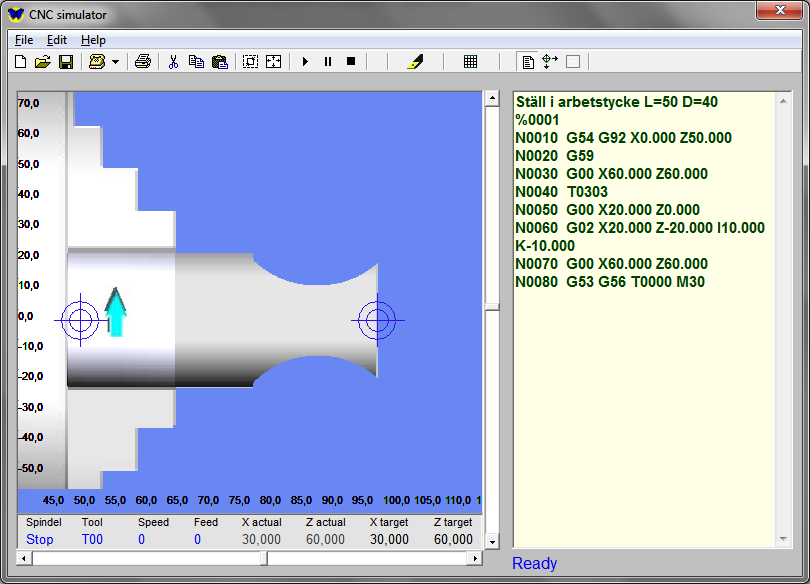
\includegraphics[width=.65\linewidth]{1.png}
    \caption{Построение заданной дуги\label{fig:default}}
\end{figure}

\begin{figure}[ht]
\centering
	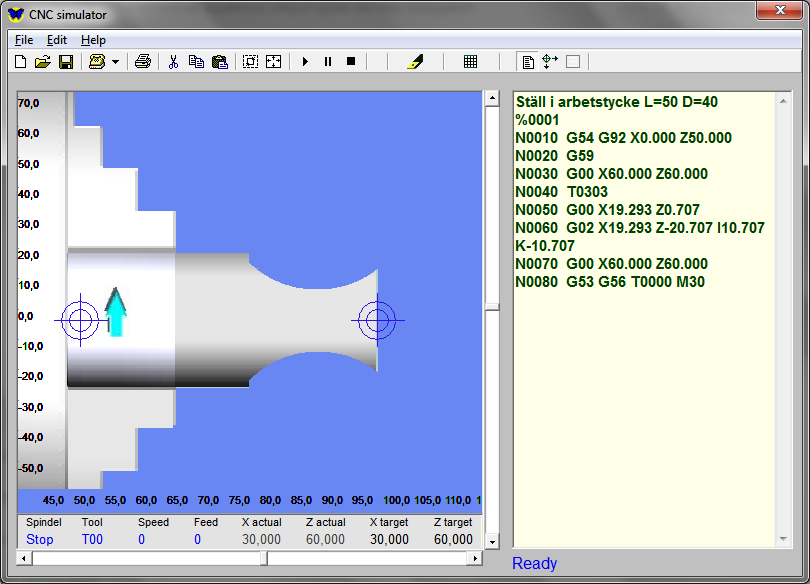
\includegraphics[width=.65\linewidth]{2.png}
    \caption{Построение дуги с измененным радиусом (на 1 мм больше стандартного)\label{fig:changed}}
\end{figure}

\begin{figure}[ht]
\centering
	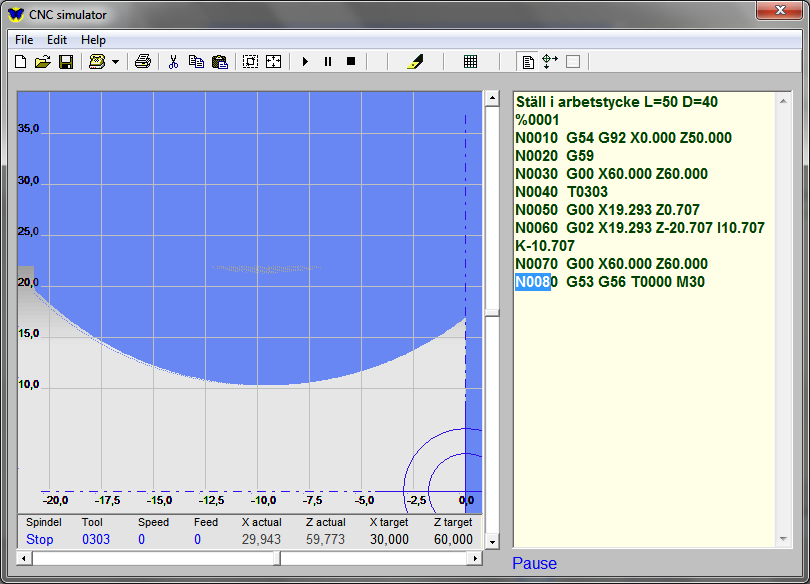
\includegraphics[width=.9\linewidth]{3.png}
    \caption{Дуга с измененным радиусом в масштабе\label{fig:closeup}}
\end{figure}

\begin{figure}[ht]
\centering
	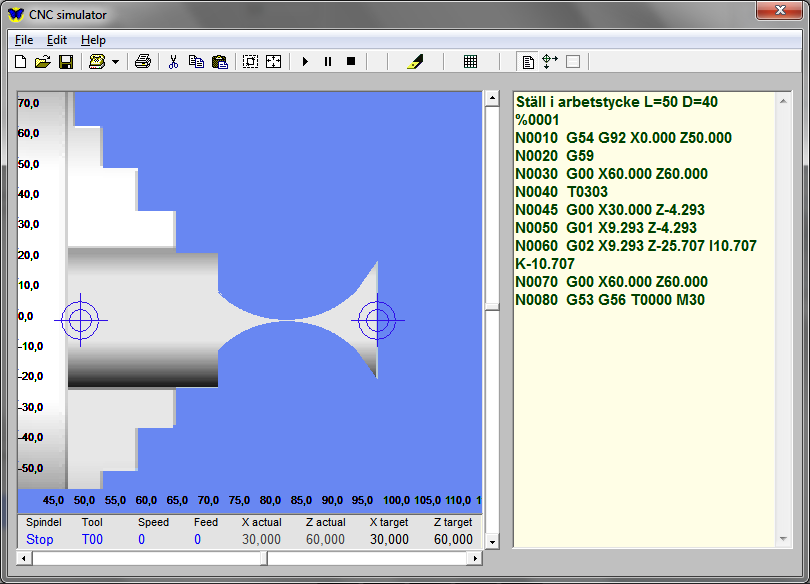
\includegraphics[width=.9\linewidth]{4.png}
    \caption{Неправильное построение дуги (смещение по оси Z)\label{fig:changedz}}
\end{figure}

\begin{figure}[ht]
\centering
	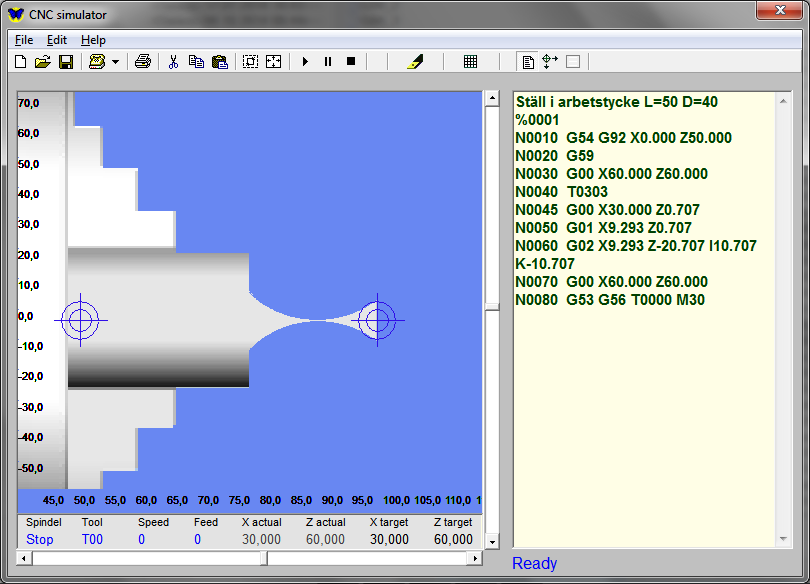
\includegraphics[width=.9\linewidth]{5.png}
    \caption{Дуга с другим центром (смещение только по оси X)\label{fig:changedx}}
\end{figure}

\begin{figure}[ht]
\centering
	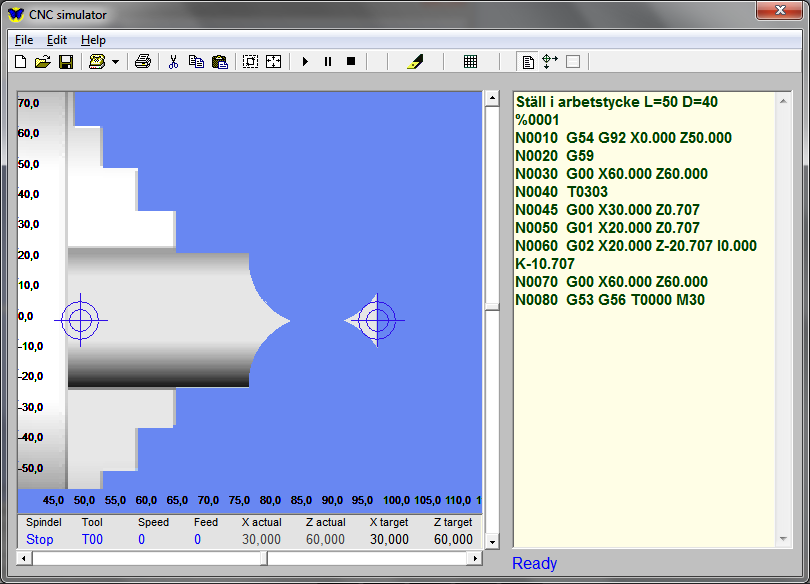
\includegraphics[width=.9\linewidth]{6.png}
    \caption{Полуокружность\label{fig:half}}
\end{figure}

\clearpage
